\documentclass[a4paper]{article}
%\usepackage[T1]{fontenc}
\usepackage[english]{babel}

\usepackage{amsmath}
\usepackage{amssymb,amsfonts,textcomp, graphicx}
\usepackage{graphics}

\usepackage{wrapfig}

\usepackage{parskip}

\usepackage{color}
\usepackage{array}
\usepackage{hhline}
\usepackage{subcaption}

\usepackage{textcomp}

\usepackage[hidelinks]{hyperref}

\setlength\tabcolsep{1mm}
\renewcommand\arraystretch{1.3}

\setlength\voffset{-1in}
\setlength\hoffset{-1in}
\setlength\topmargin{0.7874in}
\setlength\oddsidemargin{0.7874in}
\setlength\textheight{10.118099in}
\setlength\textwidth{6.6932993in}
\setlength\footskip{0.0cm}
\setlength\headheight{0cm}
\setlength\headsep{0cm}


\begin{document}

\newcommand\textstyleEmphasis[1]{\textit{#1}}
\renewcommand{\contentsname}{Table des mati\`eres}
\renewcommand\refname{R\'ef\'erences}

\renewcommand{\abstractname}{Pr\'eambule}
\title{\textbf{Simulation \'electromagn\'etique \\ et techniques de mesure RF}}
\author{Mohamed Hage Hassan \\ Cl\'ement Cheung}
\date{9 Octobre 2017}
\maketitle
\thispagestyle{empty}


\iffalse
\clearpage
\fi

\tableofcontents
\clearpage

\iffalse

\begin{figure}[!htb]
\begin{center}
  \includegraphics[scale=0.47]{Echantillonneur-bloqueur.png}
  \caption{Sch\'ema d'un \'echantilloneur-bloqueur \`a capacit\'e commut\'ee}
\end{center}
\end{figure}

\fi

\section{Introduction}
L'objectif principal de ce TP porte sur l'initiation \`a l'utilisation avanc\'ee d'ADS, et comprend une s\'erie de
 manipulations pour comprendre l'efficacit\'e de cet outil \`a effectuer des diff\'erents genres de simulations,
 aux niveaux \'electromagn\'etique ou sch\'ematique. Ces d\'emarche vont \^etre primordiales pour la r\'ealisation du projet
 de l'interface Wi-Fi que l'on r\'ealise en parall\`ele.\\


Les diff\'erents r\'esultats de simulations vont \^etre interpr\'et\'es, en partant d'une \'etude d'un filtre d'ordre 5
en technologie microruban, puis par l'analyse d'une antenne patch miniature, avec la synth\`ese semi-automatique de
mod\`ele de filtres connus, et finalement par le processus du de-embedding et les techniques de mesure radiofr\'equences.

\section{Filtre d'ordre 5}

Nous commen\c cons par l'\'etude d'un filtre microruban passe-bas d'ordre 5.
Il est compos\'e 3 inductances en s\'erie dans les lignes de propagation fines et de 2 capacit\'es en parall\`ele dans les lignes plus larges.
Le schematic suivant est issu de ADS.

\begin{figure}[!htb]
\begin{center}
  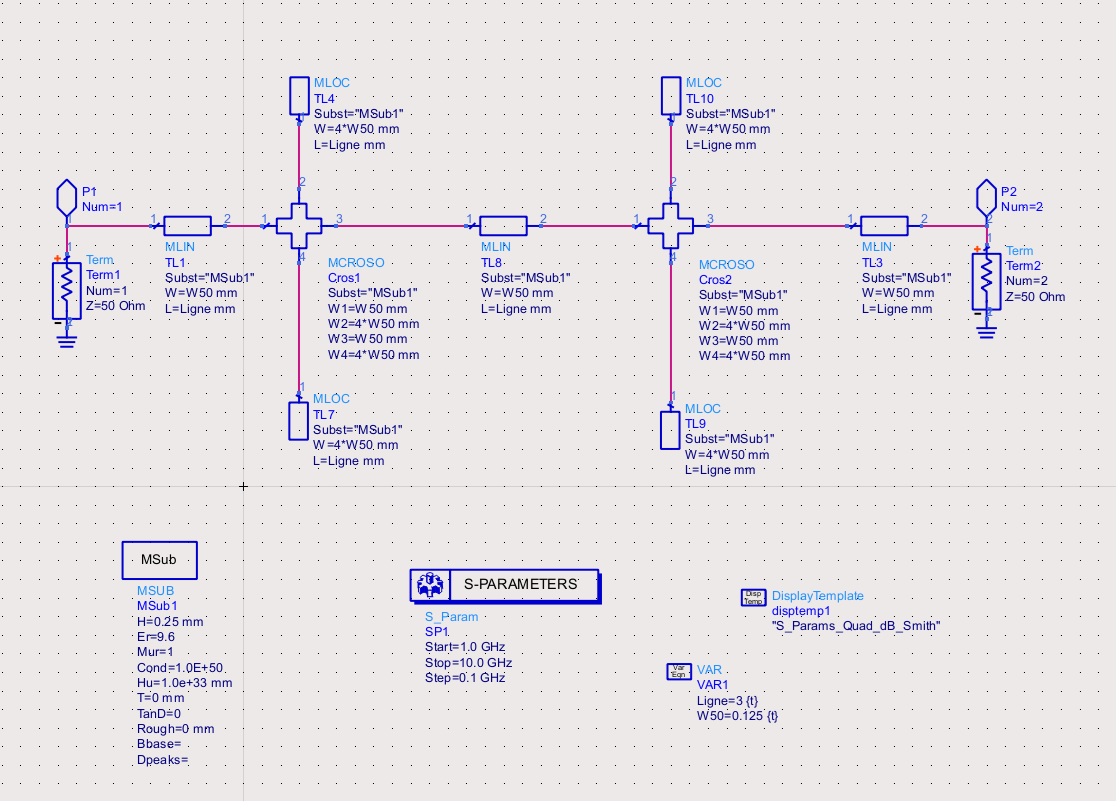
\includegraphics[scale=0.43]{general_schematic.png}
  \caption{Simulation primaire d'un filtre microruban}
\end{center}
\end{figure}

Nous avons utilis\'e les \'el\'ements MCROS $\&$ MLOC pour construire les lignes larges au lieu d'un \'el\'ement simple car cela
 permet de mieux voir le couplage entre les 2 lignes par la suite quand la longueur des lignes fines va varier.
Les simulations s'effectuent avec les \'el\'ements TERM \`a $Z=50 \Omega$ ainsi que la bo\^ite S-PARAM qui va permettre de r\'ecup\'erer
les param\`etres S pour une variation en fr\'equence entre 1 \`a 10GHz de notre filtre.

L'objectif est de r\'ealiser l'adaptation du filtre \`a $50 \Omega$  ($S_{11} = -20 dB$). Les longueurs totales W $\&$ L de la ligne
ont d'abord \'et\'e fix\'ees de mani\`ere \`a avoir $f_0 = 5 GHz$ et $E_{eff} = 90^{\circ}$ environ avec $W=0.25 mm$ et $L = 5.88mm$.
Le reste des longueurs de chaque brin est ensuite param\'etrable.

Nous verrons par la suite que la longueur du brin central TL8 aura des cons\'equences sur
la fr\'equence de r\'esonance en entr\'ee et sur l'adaptation du filtre.


\iffalse
On d\'esire r\'ealiser une adapation du filtre au en consid\'erant le coefficient de r\'eflexion $S_{11}$ \`a l'entr\'ee du filtre.
(On aura une adaptation du filtre pour $S_{11} = - 20 db $ min en entr\'ee).
Les valeurs W et L de la ligne sont param\'etrables, on verra plus tard que la manipulation de la longeur du brin central du filtre
\`a des conc\'esquences sur la fr\'equence de r\'esonance en entr\'ee, et aussi celle de l'adaptation.
\fi

Les premi\`eres simulations permet de montrer que l'effet de couplage \'electromang\'etiques entres les blocs capacitifs du filtres
(TL4, TL10 et TL7, TL9 sur la figure 1), n'est pas pris en compte. Il faut ainsi essayer d'appliquer une mod\'elisation EM,
en passant par :
\begin{itemize} \itemsep -3pt
  \item [-] Simulation du schematic.
  \item [-] Dessin du composant (layout).
  \item [-] Ex\'ecution d'un rafinement du sch\'ema en mechs de 3 cellules par largeur.
  \item [-] Essais de simulations pour un symbol cr\'ee \`a partir du mech.
  \item [-] Changement du mat\'eriel pour le filtre d'un conducteur parfait vers le cuivre, et sa simulation.
  \item[-] Simulation avec un symbol en "emModel" ou simulation \'electromagn\'etique.
\end{itemize}

\subsection{Mod\'elisation des mailles et simulation du schematic}
Nous cr\'eons le layout \`a partir du schematic pr\'ec\'edent et on effectue un maillage (mesh) pour
effectuer les simulations EM des moments (momentum) :

\begin{figure}[!htb]
\begin{center}
  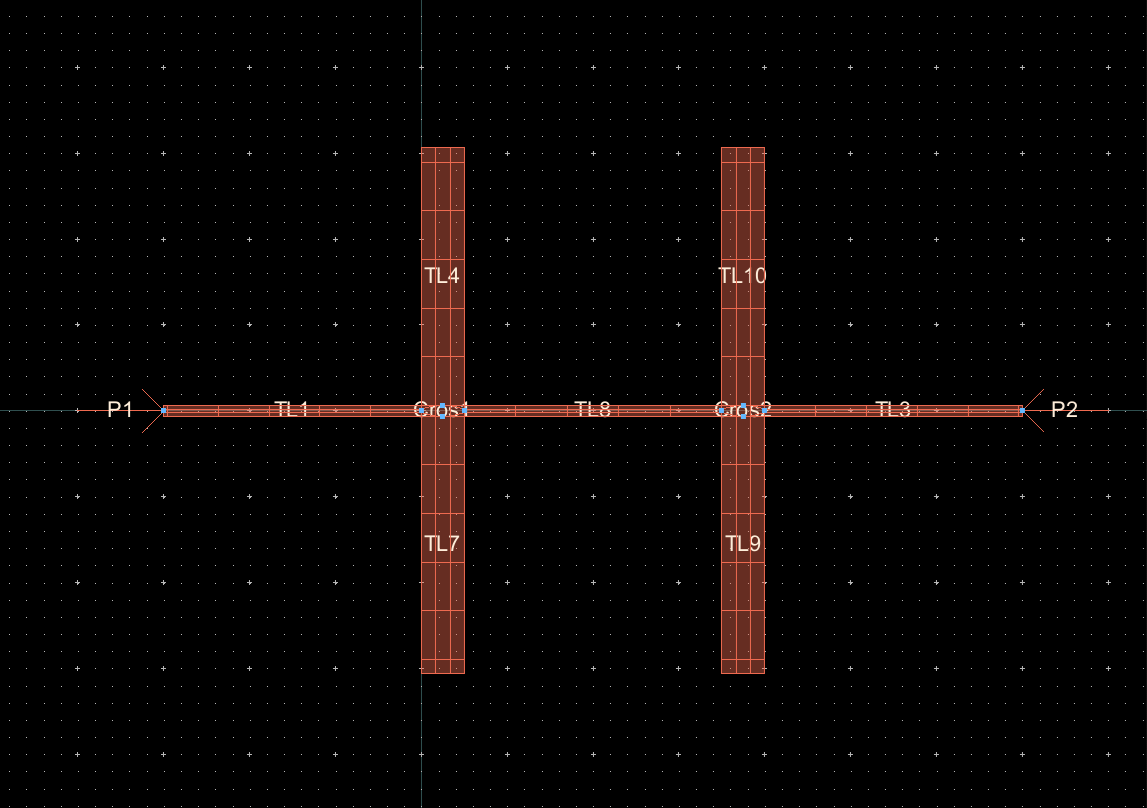
\includegraphics[scale=0.35]{filter_layout.png}
  \caption{Dessin et raffinement du layout}
\end{center}
\end{figure}

Suite \`a la simulation nous obtenons le graphe fig.\ref{sim_schematic_momentum} o\`u les r\'esultats des simulations
schematic sont superpos\'es aux layout.


Les param\`etres $S_{21}$ de chacune des simulations indiquent le comportement passe-bas du filtre. \`A $4 GHz$,
nous avons apparament une tr\`es bonne adaptation, \`a la r\'esonance, \`a plus que $-20 db$ en entr\'ee pour les deux mod\`eles.
\\
Une simulation EM est n\'ecessaire pour voir l'effet du couplage des condensateurs.\\

Le mod\`ele schematic semble avoir une d\'eviation l\'eg\`ere par rapport \`a celui qui est maill\'e.
Une bonne adaptation en entr\'ee indique que toute la puissance \'etait transf\'er\'ee \`a la charge, sachant que l'on garde
un minimum de r\'eflexion.

\clearpage

\begin{figure}[!htb]
\begin{center}
  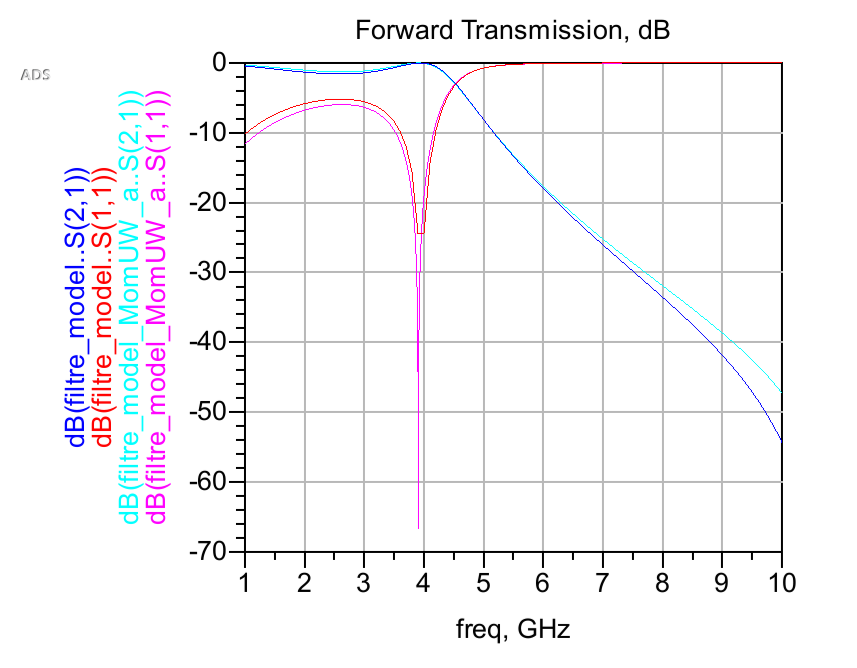
\includegraphics[scale=0.35]{schematic_mesh.png}
  \caption{Simulation du schematic et du mesh g\'en\'er\'e (filtre\_model et model\_MomUW) respectivement.}
  \label{sim_schematic_momentum}
\end{center}
\end{figure}


\subsection{Simulation avec le cuivre}
Cette fois, nous rempla\c cons le conducteur parfait du layout par du cuivre et relan\c cons la m\^eme simulation que pr\'ec\'edemment.
Les courbes cyan $\&$ rose correspondent \`a la simulation conducteur parfait et les courbes bleu $\&$ rouge au cuivre, repr\'esent\'es
par la figure \ref{sim_momentum_copper}.

\begin{figure}[!htb]
\begin{center}
  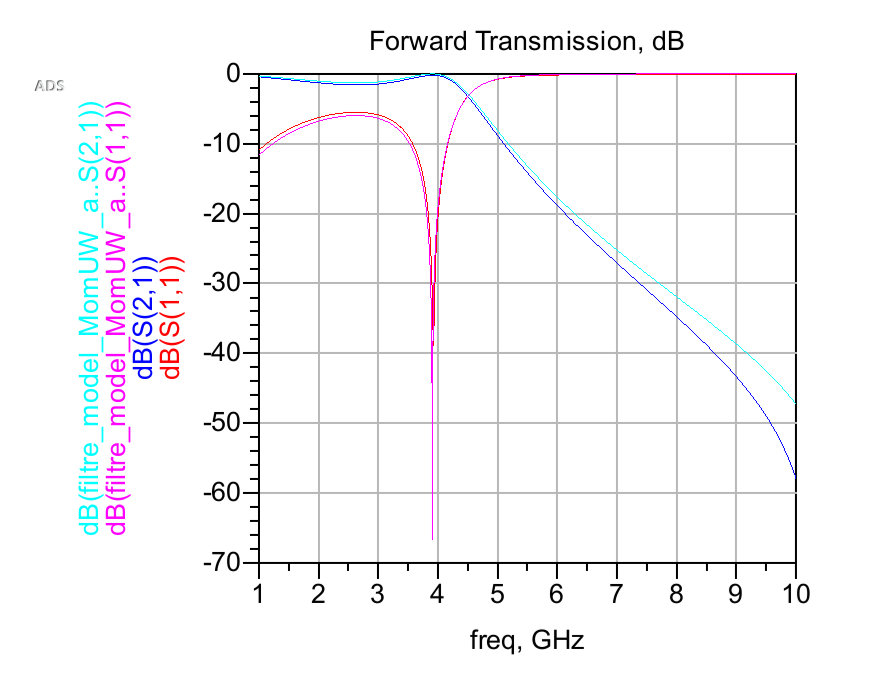
\includegraphics[scale=0.35]{mesh_copper.png}
  \caption{Simulation du mesh g\'en\'er\'e avec celui en copper}
  \label{sim_momentum_copper}
\end{center}
\end{figure}

Les diff\'erences observ\'ees sont minimes sauf \`a haute fr\'equence o\`u la pente du filtre au cuivre est l\'eg\`erement plus importante.\\
Nos simulations n'ont pas rendu compte de diff\'erences majeures entre ces deux mod\`eles. La figure \ref{sim_3D} montre la vue 3D de
notre filtre microruban.

\begin{figure}[!htb]
\begin{center}
  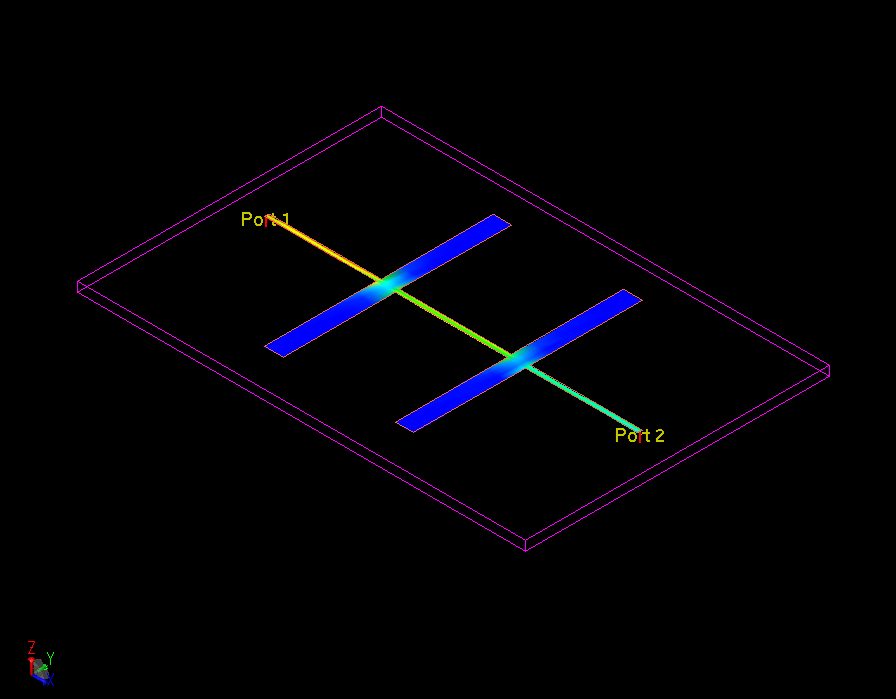
\includegraphics[scale=0.30]{3D_electromag_sim.png}
  \caption{Simulation \'electromagn\'etique en 3D}
  \label{sim_3D}
\end{center}
\end{figure}

On remarque que les zones en orange pr\'esentent l'onde EM confin\'ee dans la ligne de transmission fine et qu'elle s'\'etend au
passage des lignes larges (bleu).

\subsection{G\'eneration d'un symbol et simulation \'electromagn\'etique}

L'\'etape suivante \'etait de cr\'eer un symbole de notre filtre dans ADS afin de pouvoir continuer plus facilement les simulations.

\begin{figure}[!htb]
  \begin{subfigure}[t]{.5\linewidth}
      \centering
      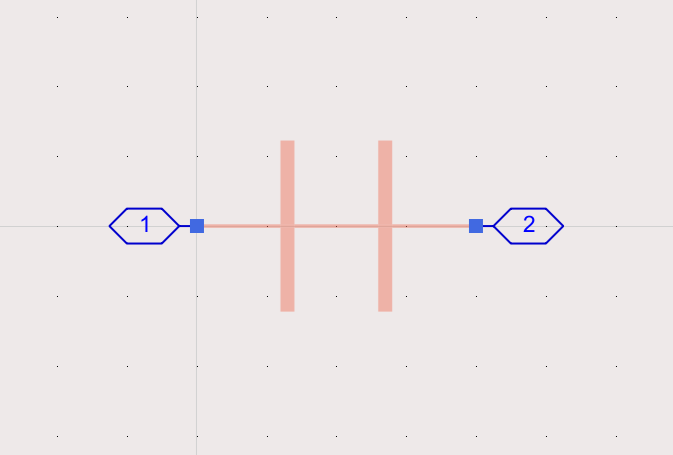
\includegraphics[width=0.99\linewidth]{auto_generated_schematic_copper.png}
      %\caption{De-embedding en open}
      \label{fig:auto_generated_schematic_copper}
  \end{subfigure}%
  \begin{subfigure}[t]{.5\linewidth}
    \centering
    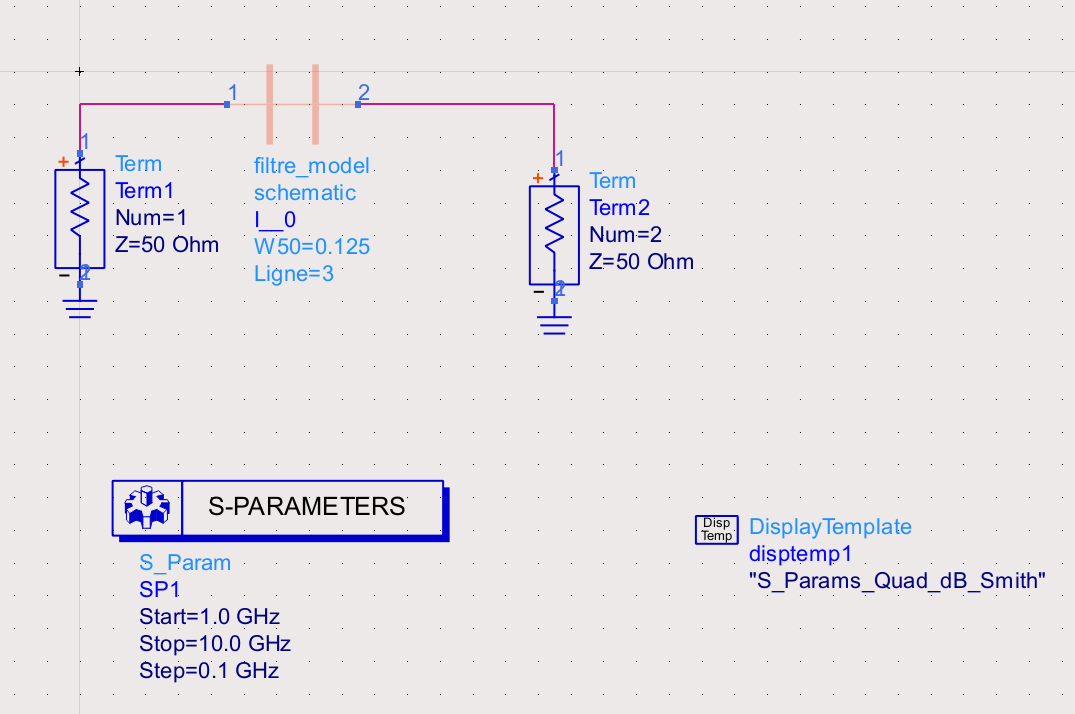
\includegraphics[width=1\linewidth]{filtre_symbol.png}
    %\caption{De-embedding en short}
    \label{fig:filtre_symbol}
  \end{subfigure}%
  \caption{Sch\'ema du symbol auto-g\'en\'er\'e et le bench respectivement}
  \label{fig:filtre_symbol_bench}
\end{figure}

Nous avons d\'efini des variables globales pour la longueur Ligne et W50 que nous pouvons ensuite balayer pour obtenir
diff\'erentes fr\'equences de coupure du filtre. \\
Nous avons fait un sweep sur la variable Ligne de 1 \`a $6 mm$ par pas de $1 mm$.
Le r\'esultat est pr\'esent\'e sur le graphe fig. \ref{sim_Electromagnetic}.\\

L'analyse de ces courbes montre que l'on est toujours adapt\'e \`a $50 \Omega$  sur la plage de fr\'equence $[1 ; 10 GHz]$ quelque soit la longueur de ligne.
On remarque cependant que la fr\'equence de coupure (et d'adaptation) sur les courbes rouges baisse plus la longueur de ligne est importante.\\

Cela est d\^u au comportement inductif d'un long filtre sans couplage capacitif entre les deux lignes larges. On sera ainsi plus pr\`es du mod\`ele
schematic qui ne prend pas en compte ces effets.\\

\clearpage
\begin{figure}[!htb]
\begin{center}
  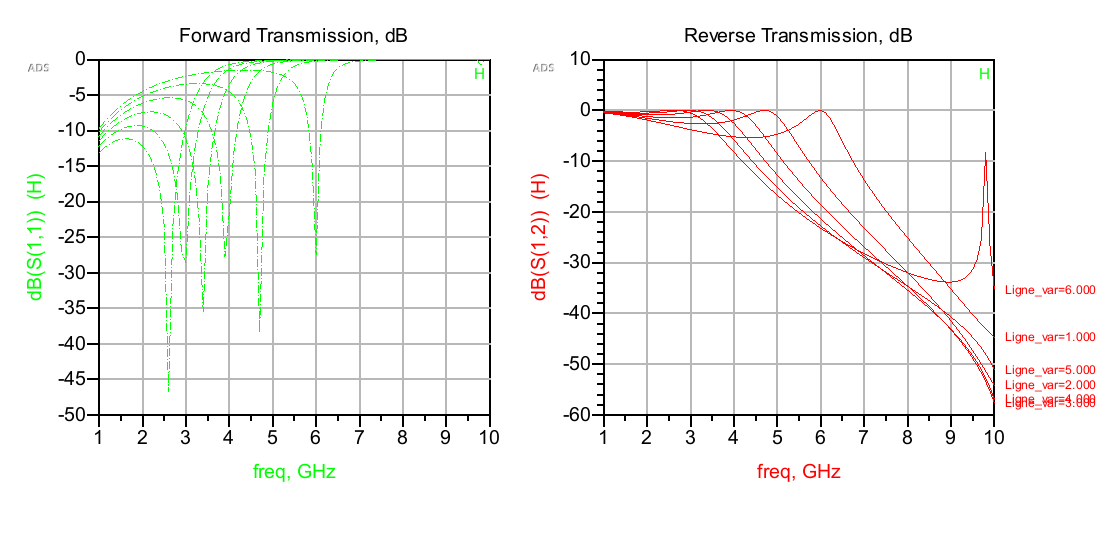
\includegraphics[scale=0.45]{Simulation-Finale-Globale-EM.png}
  \caption{Simulation \'electromagn\'etique du Symbole (en copper)}
  \label{sim_Electromagnetic}
\end{center}
\end{figure}

\section{Antenne miniature patch}
\subsection{Conception d'une antenne miniature et simulation}

Dans cette partie nous avons r\'ealis\'e une antenne patch miniature sur substrat. Le layout pr\'esent\'e fig.\ref{patch_antenna} montre le port d'acc\`es
central ainsi que les 2 bras lat\'eraux qui ont une longueur variable selon l'adaptation voulue.
\begin{figure}[!htb]
\begin{center}
  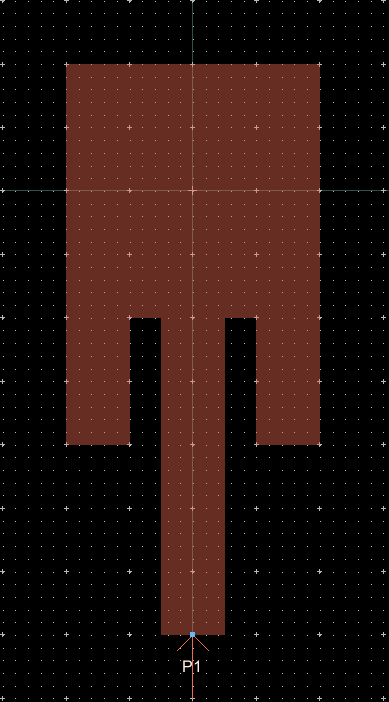
\includegraphics[scale=0.35]{patch_antenna.png}
  \caption{Layout de l'antenne patch}
  \label{patch_antenna}
\end{center}
\end{figure}

Nous avons ensuite lanc\'e une premi\`ere simulation EM de ce layout (fig.\ref{Simulation-Layout-Antenne-EM}) pour v\'erifier grossi\`erement l'adaptation de notre antenne.
On voit ici qu'elle n'est pas tr\`es bien adapt\'ee \`a $f = 9 GHz$ pour le moment ($S_{11} > -20dB$).
\clearpage

\begin{figure}[!htb]
\begin{center}
  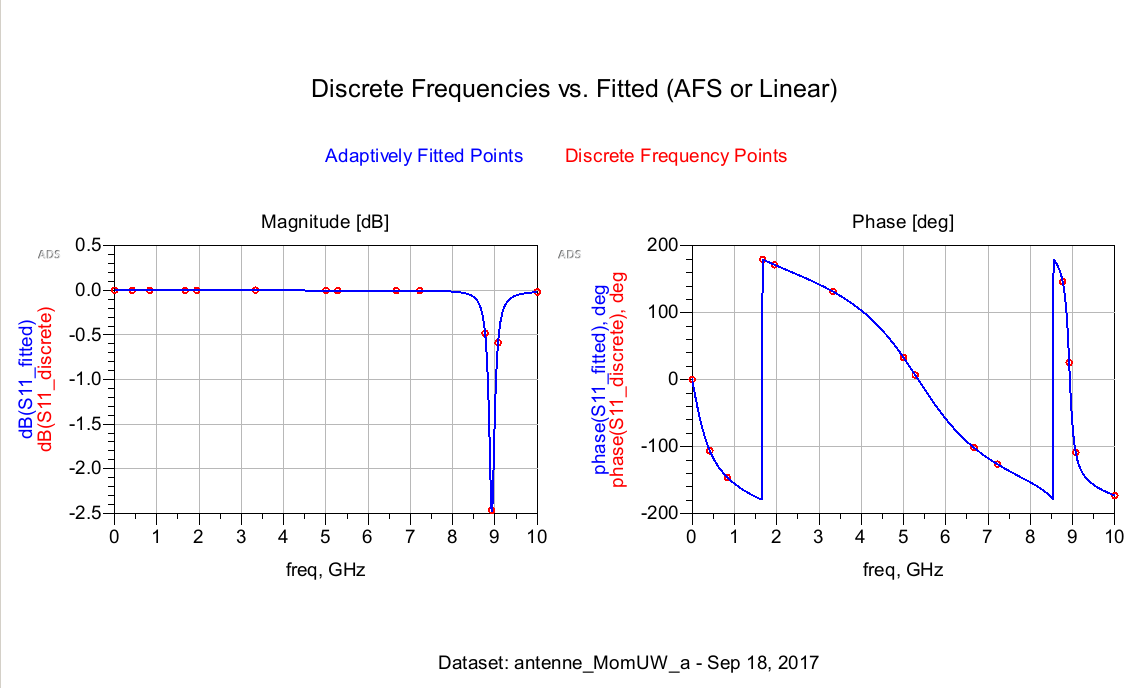
\includegraphics[scale=0.42]{Simulation-Layout-Antenne-EM.png}
  \caption{Simulations discr\`ete}
  \label{Simulation-Layout-Antenne-EM}
\end{center}
\end{figure}

Nous avons ensuite r\'ealis\'e un symbole ADS de l'antenne (fig.\ref{schematic_antenne_simu}) pour comparer avec les simulations Momentum du layout.

\begin{figure}[!htb]
\begin{center}
  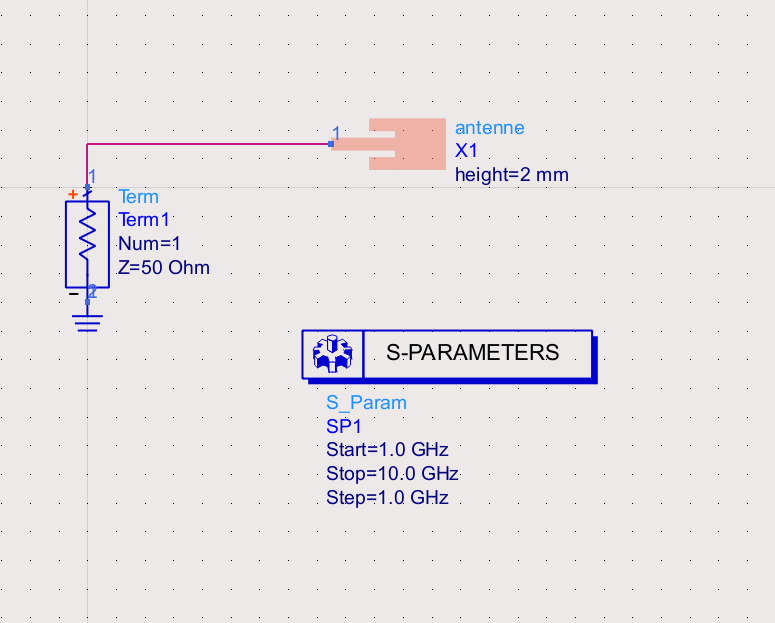
\includegraphics[scale=0.37]{schematic_antenne_simu.png}
  \caption{Sch\'ematic de l'antenne patch}
  \label{schematic_antenne_simu}
\end{center}
\end{figure}

Le graphe fig.\ref{height_2_3mm} montre la simulation schematic (rouge) versus la simulation momentum (bleu) pour une m\^eme longueur
de bras height = 2.3mm. \\
On remarque directement une moins bonne adaptation et un d\'ecalage vers les hautes fr\'equences
car le mod\`ele EM prend en compte les effets capacitifs parasites entre les bras et le port d'acc\`es principal de l'antenne.
\clearpage
\begin{figure}[!htb]
\begin{center}
  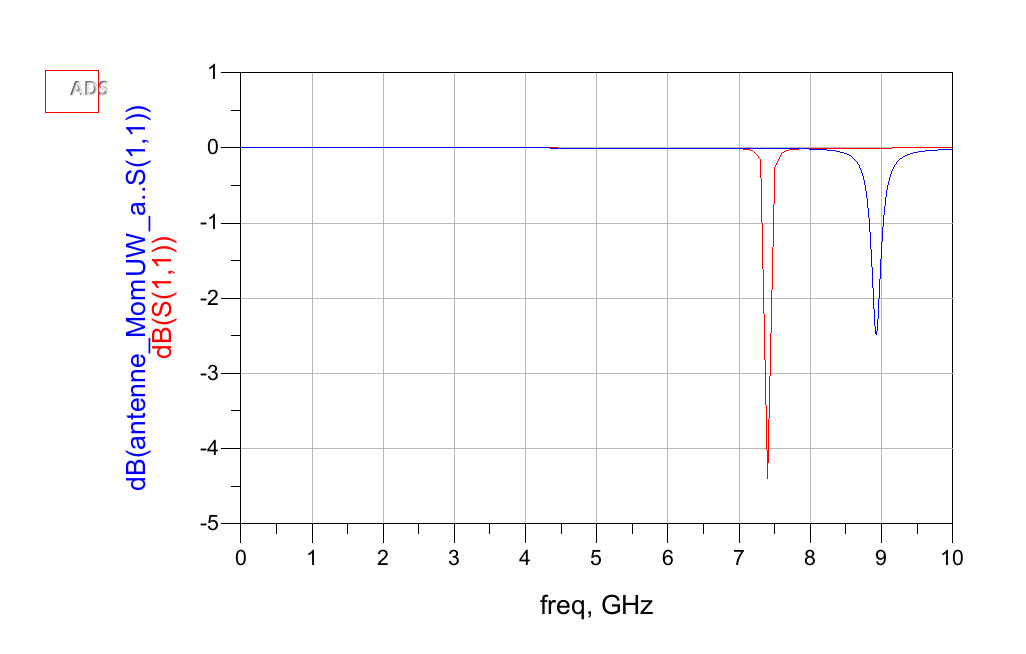
\includegraphics[scale=0.45]{height_2_3mm.png}
  \caption{Simulation pour une longeur de bras $h = 2.3 mm$}
  \label{height_2_3mm}
\end{center}
\end{figure}

Nous avons ensuite utilis\'e le tuner pour trouver la longueur de bras d'antenne qui donnait une adaptation \`a $-20dB$ minimum en cr\'eant un param\`etre de variation dans le layout.
Nous avons trouv\'e que la valeur height $h = 1.31 mm$ donnait le r\'esultat le plus int\'eressant (point M1 sur le graphe fig.\ref{adaptation_height_1-31mm}) pour l'adaptation.

\begin{figure}[!htb]
\begin{center}
  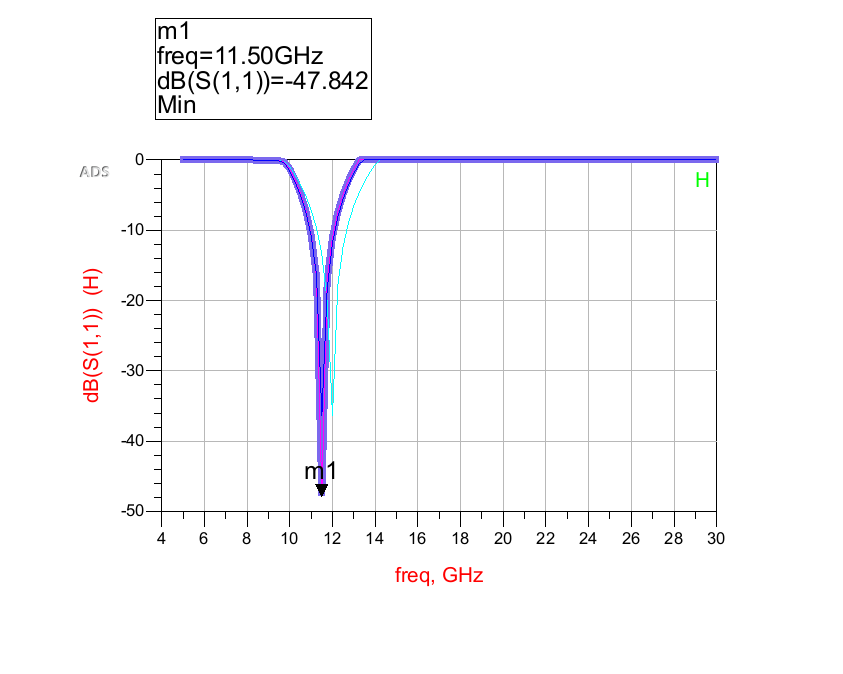
\includegraphics[scale=0.45]{adaptation_height_1-31mm.png}
  \caption{Simulation pour une longeur de bras $h = 1.31 mm$ (maximum d'adaptation)}
  \label{adaptation_height_1-31mm}
\end{center}
\end{figure}

\clearpage
\subsection{G\'en\'eration automatique des composants passifs}
Sous ADS, il est possible de commander le logiciel pour cr\'eer des composants passifs (coupleurs, filtres..).
En utilisant DesignGuide, on sp\'ecifie les param\`etres n\'ecessaires pour le logiciel (fr\'equence de coupure,
pente de - n db/d\'ecade). DesignGuide va synth\'etiser un \'el\'ement passif en indiquant son ordre.

L'un des \'el\'ements synth\'etis\'e est un coupleur hybride :

\begin{figure}[!htb]
\begin{center}
  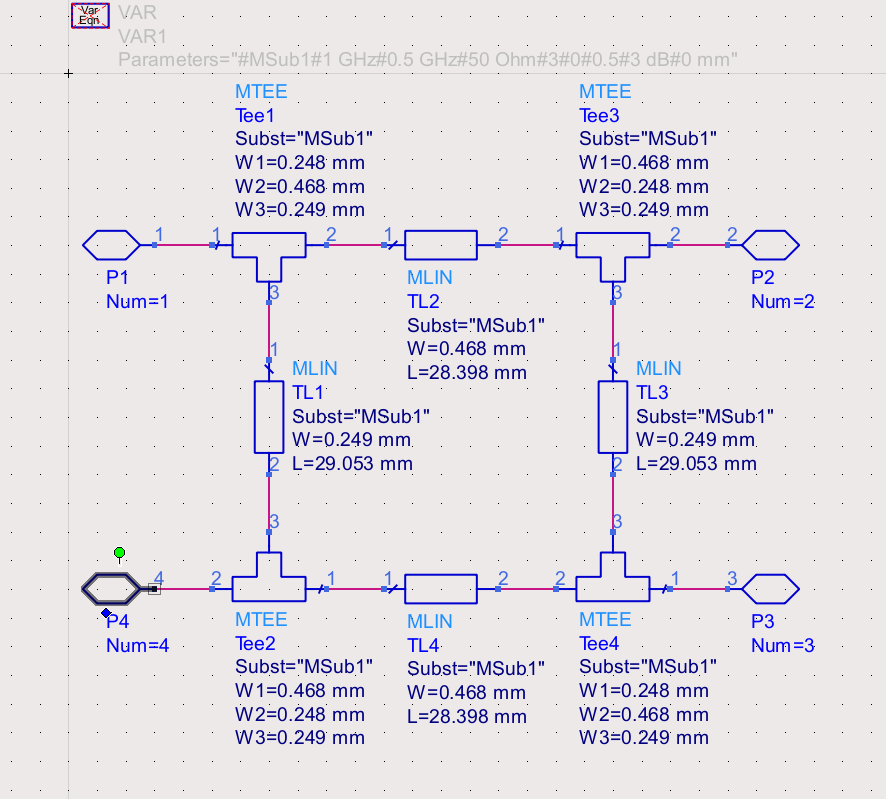
\includegraphics[scale=0.30]{Coupleur-Hybride-Synthese.png}
  \caption{Sch\'ema d'un coupleur hybride auto-g\'en\'er\'e}
  \label{Coupleur-Hybride-Synthese}
\end{center}
\end{figure}

Une analyse des param\`etres W et L de chacun des brins du coupleur permet de v\'erifier que le sch\'ema
de synth\`ese rempli bien les sp\'ecifications (imp\'edance caract\'eristique du brin $= Z_0$ ou $ \sqrt{2}/2 Z_0$).
Les coefficients de r\'eflexion pour chacune des voies sont analys\'es : on voit qu'il y a une adaptation totale
en entr\'ee des ports 1 et 4 (\`a $-40 db$) et une r\'eflexion importante par rapport aux entr\'ees des ports 2 et 3.
C'est li\'e aux caract\'eristiques du coupleur (passage en port 4 et r\'ejection totale d'une onde incidente en 1 vers les
ports 2 et 3).

\begin{figure}[!htb]
\begin{center}
  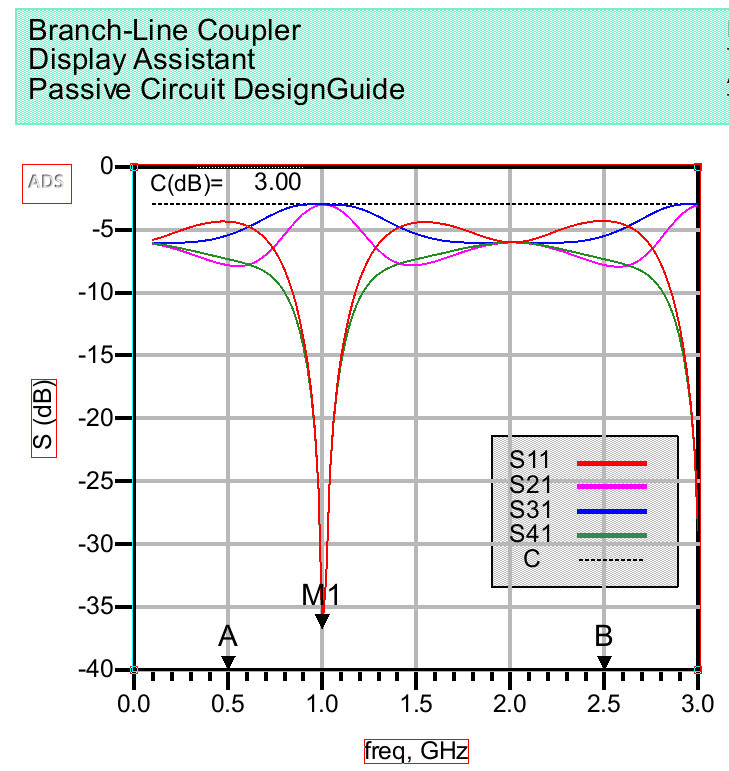
\includegraphics[scale=0.35]{Coupleur-Simulation-resultat.png}
  \caption{Simulation du coupleur hybride}
  \label{Coupleur-Simulation-resultat}
\end{center}
\end{figure}


\clearpage
\section{Techniques de mesures RF et de-embedding}
\subsection{Analyse des m\'ethodes du de-embedding}
Le calibrage peut s'effectuer g\'en\'eralement selon deux m\'ethodes :

\subsubsection{Calibrage ex-situ}
\textbf{SOLT : Short Open Line Transition calibration} \\
Ce type de calibrage est commercial, et d\'epend de la pr\'ecision des valeurs indiqu\'es par le fabriquant.
L'utilisation de ce type de calibrage entraine la n\'ecessit\'e de conna\^itre les standards fournis, ainsi
que 12 termes d'erreurs \`a retrouver.
Les carat\'eristiques g\'en\'erales se r\'esument par :
\begin{itemize}
  \item[-] Rien \`a r\'egler du cot\'e de l'analyseur vectoriel (pas d'algorithme).
  \item[-] Proc\'edure de calibrage particuli\`erement longue.
  \item[-] N\'ecessite une intervention de de-embedding.
\end{itemize}

La partie de de-embedding consiste donc de passer du plan de mesure (les PADs) vers le plan du DUT.
Les PADs sont utilis\'es pour les connecteurs wafer car les lignes d'acc\`es permettent d'\'eviter le couplage
entre 2 lignes si le DUT est petit et pour laisser le temps \`a l'onde d'excitation de l'analyseur vectoriel
de s'\'etablir correctement.

\subsubsection{Calibrage in-situ}
\textbf{TRL : Thru Reflect Line } \\
Ce type de calibrage repose sur l'autocalibration, et c'est nous m\^eme qui le fabriquons (m\'ethode maison).
Le calibrage s'effectue, contrairement au calibrage SOLT, directement au plan du DUT, et ne n\'ecessite la connaissance
que de 8 termes d'erreurs.

\subsection{\'Etude th\'eorique}

\begin{figure}[!htb]
\begin{center}
  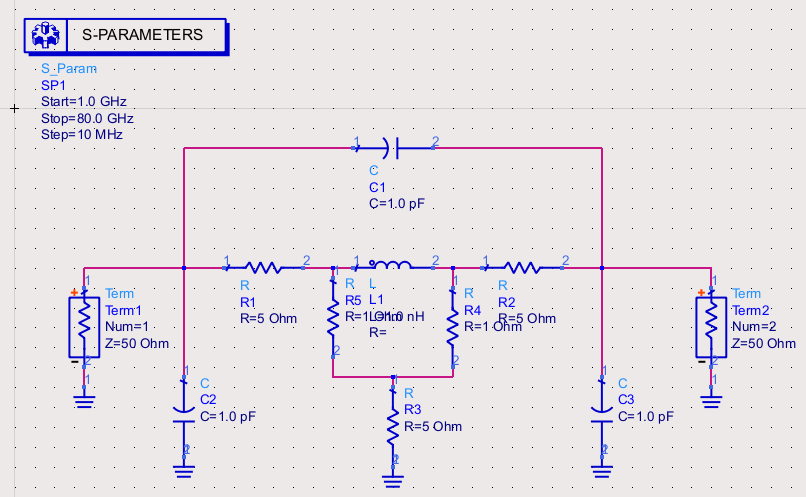
\includegraphics[scale=0.45]{de-embedding_scheme.png}
  \caption{Mod\'elisation des parasites en \'el\'ements discrets }
  \label{de-embedding-scheme}
\end{center}
\end{figure}

Notre but c'est de retrouver $Y_{DUT}$, ou m\^eme $S_{DUT}$ du circuit ou de l'\'el\'ement sous test, ici un pont en $\Pi$.
On utilise la m\'ethode short-open de-embedding, qui consiste \`a enlever les parasites (fig. \ref{de-embedding-scheme}) par un essai de 2 types de terminaisons :
court-circuit, puis circuit-ouvert. Rappelons que\cite{sim-elec-cours}:
\[
Y_{openpad} = Y_{Mesure} - Y_{open}
\]
 \clearpage
 \[
Y_{shortpad} = Y_{short} - Y_{open}
\]
et surtout :
\[
Z_{DUT} = Z_{openpad} - Z_{shortpad}
\]
ce qui implique que :
\[
Y_{DUT} = \bigg( \big( Y_{openpad} \big)^{-1} - \big( Y_{shortpad} \big)^{-1} \bigg)^{-1}
\]
Ces transformations vont \^etre cod\'ees dans un bench global pour simuler le processus de de-embedding. Une analyse va comparer
les r\'esulat des simulations entre l'\'etape de de-embedding, et une analyse de l'\'el\'ement seul:

\begin{figure}[!htb]
\begin{center}
  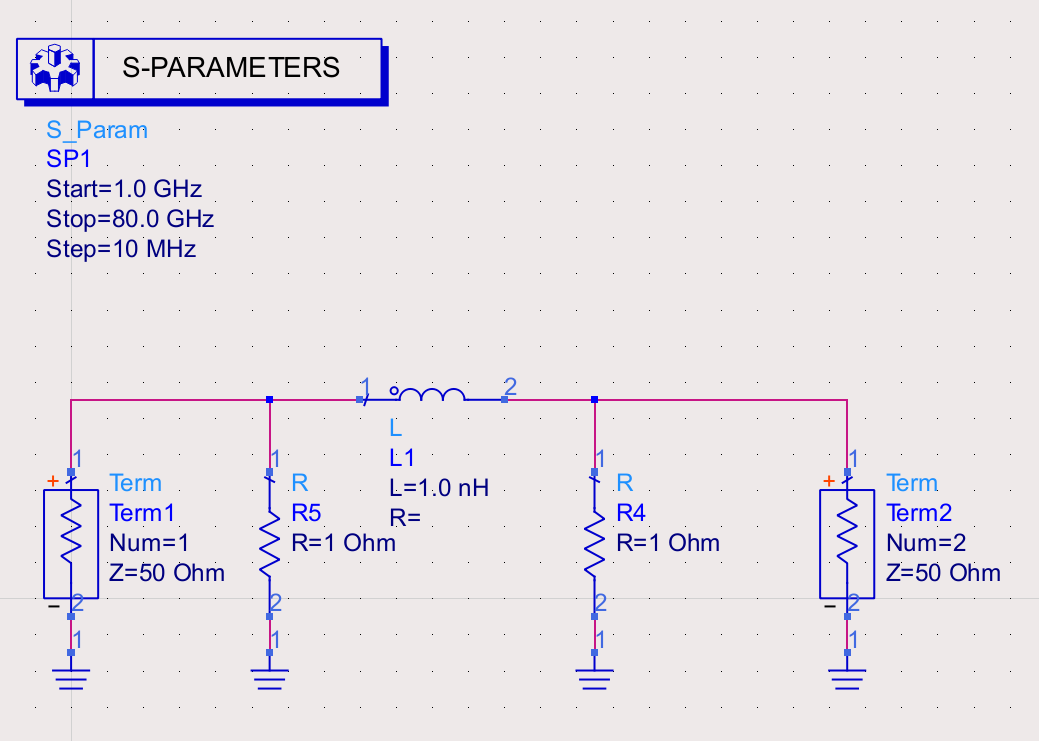
\includegraphics[scale=0.23]{de-embedding_bench.png}
  \caption{Mod\'elisation de l'\'el\'ement passif sous test}
  \label{de-embedding-bench}
\end{center}
\end{figure}

\subsection{R\'ealisation du de-embedding}
\textbf{M\'ethodologie}\\
Notre m\'ethode consiste \`a :
\begin{itemize}
  \item [-] R\'ealisation de 3 sch\'emas pour prendre en compte les terminaisons court-circuit et circuit-ouvert, ainsi que le sch\'ema
  complet.
  \item[-] Ex\'ecution de simulations pour les 2 terminaisons short et open.
  \item[-] Ins\'ertion des DACs (Data Acquisition Container) de simulations dans le sch\'ema g\'en\'eral et sa simulation,
   en consid\'erant les transformations indiqu\'ees pour arriver jusqu'a $Y_{DUT}$.
  \item[-] Comparaison du $S_{DUT}$, $Y_{DUT}$ avec une simulation du $S_{bench}$, $Y_{bench}$ d'un bench du pont en $\Pi$.
\end{itemize}

\begin{figure}[!htb]
  \begin{subfigure}[t]{.55\linewidth}
      \centering
      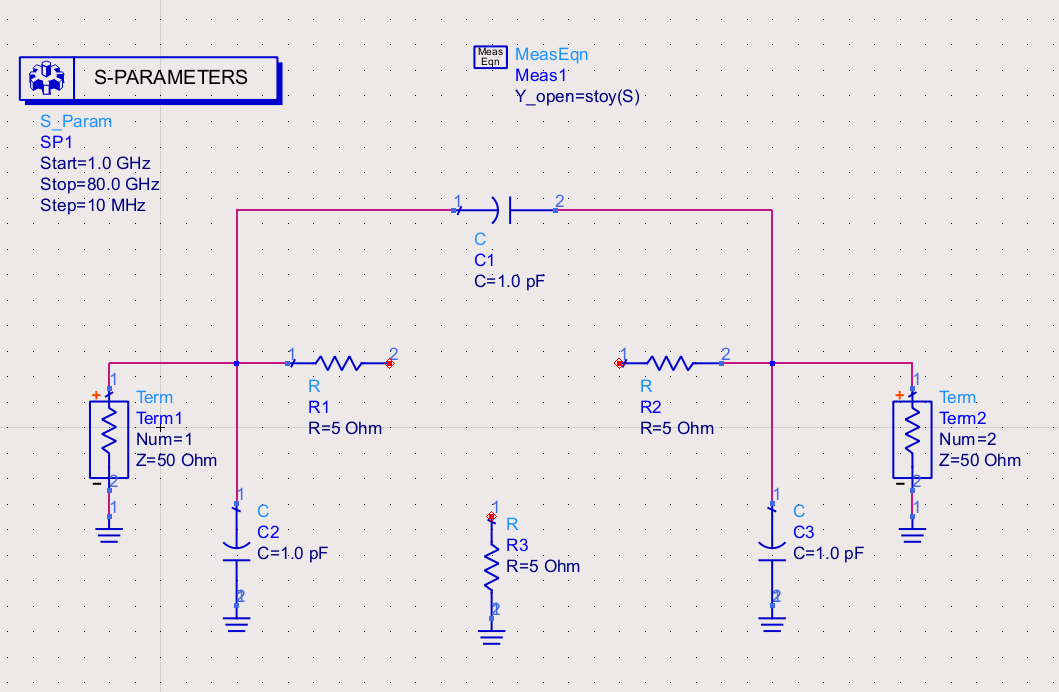
\includegraphics[width=1\linewidth]{de-embedding_open.png}
      %\caption{De-embedding en open}
      \label{fig:de-embedding-open}
  \end{subfigure}%
  \begin{subfigure}[t]{.55\linewidth}
    \centering
    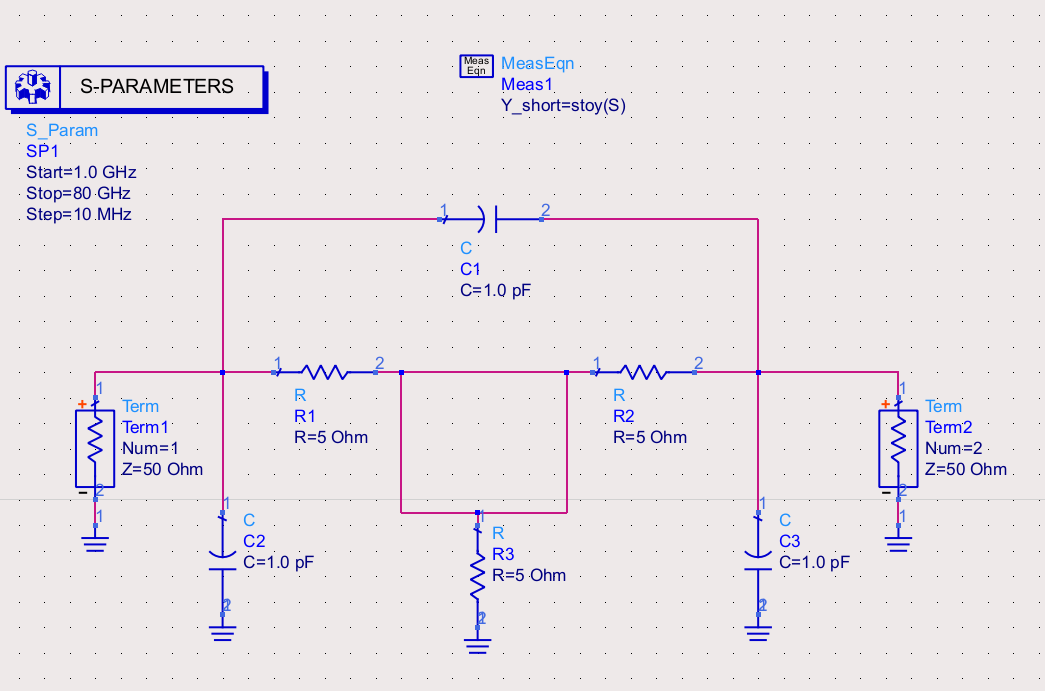
\includegraphics[width=0.99\linewidth]{de-embedding_short.png}
    %\caption{De-embedding en short}
    \label{fig:de-embedding-short}
  \end{subfigure}%
  \caption{De-embedding open et short respectivement}
  \label{fig:de-embedding Phases}
\end{figure}

\clearpage

Pour toutes les simulations, on effectue un balayage en fr\'equence entre 1 et 80 GHz pour 7901 points.

\begin{figure}[!htb]
\begin{center}
  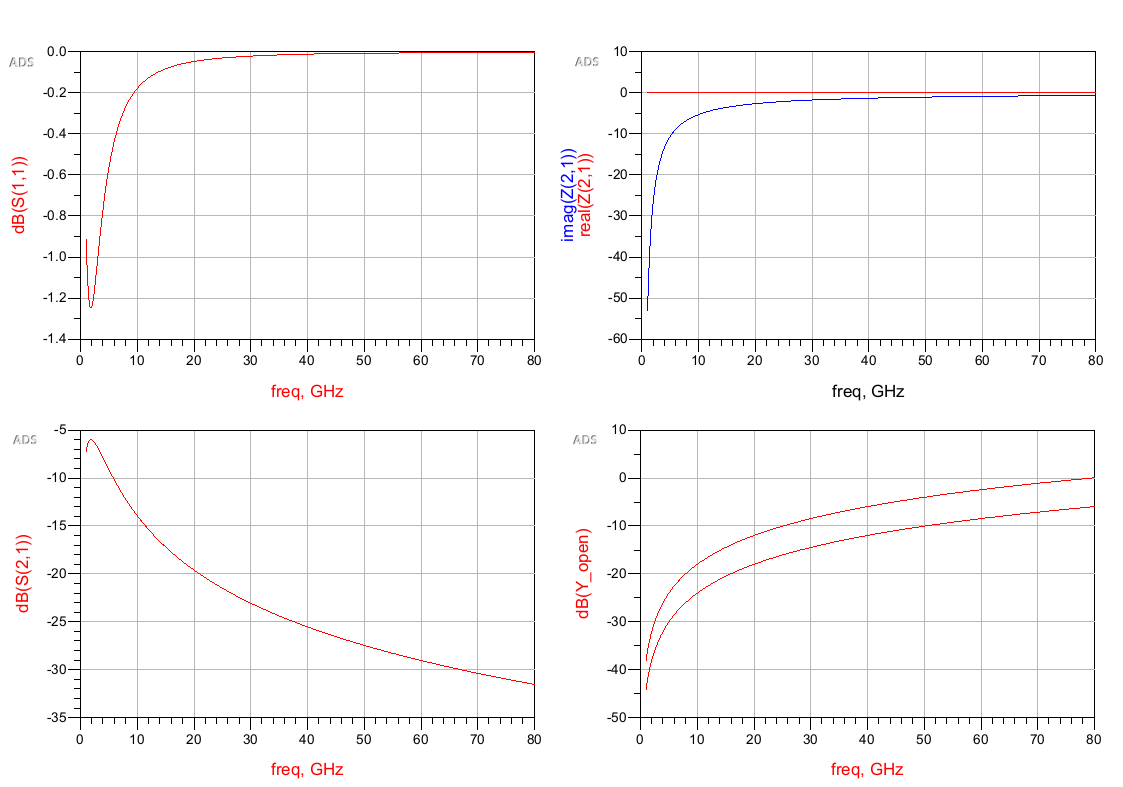
\includegraphics[scale=0.35]{de-embedding_open_sim.png}
  \caption{R\'esultat de simulation Open}
  \label{de-embedding-sim-open}
\end{center}
\end{figure}

Pour la partie open, on remarque que le circuit est assimilable \`a un pont en $\Pi$ de capacit\'es, (sans la partie
centrale), ce qui implique un comportement de filtrage : les diagrammes de $S_{11}$ et $S_{21}$ (compl\'ementaires)
montrent une attenuation de transmition en augmentation de fr\'equence. On a aussi le comportement purement r\'eactif
des capacit\'es, illustr\'e par $imag(Z_{21})$ (chute en fr\'equence).

\begin{figure}[!htb]
\begin{center}
  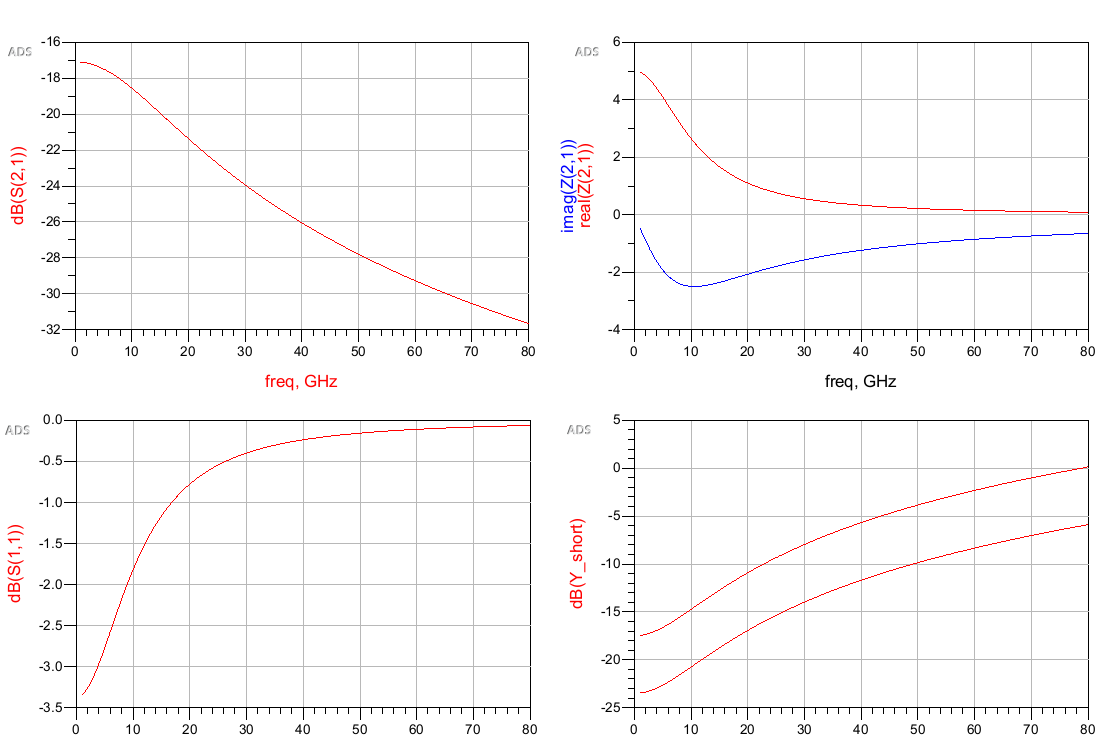
\includegraphics[scale=0.35]{de-embedding_short_sim.png}
  \caption{R\'esultat de simulation Short}
  \label{de-embedding-sim-short}
\end{center}
\end{figure}

Cependant, pour la partie short, l'\'element sous test est remplac\'e par un court-circuit : on se retouve avec l'ancienne
configuration capacitive, mais aussi avec des att\'enuation du aux r\'esistances ($R_1$, $R_2$, $R_3$) des plots d'acc\`es.
On a un ``d\'ecalage' de la fr\'equence de coupure du nouveau filtre (l'annulation de la transmition en $S_{11}$ est \`a $f= 70 GHz$).
\\
$Re\{Z_{21}\}$ indique le comportement r\'esistif du sch\'ema.\\
Sachant que le comportement en short et open du circuit repr\'esente les parasites du circuit, il faut les \'eliminer : On reprend le
mod\`ele initial et on applique les m\'ethodes math\'ematique. La robust\`esse du mod\`ele math\'ematique va indiquer l'exactitude ou
non des r\'esultats de simulation, en comparaison avec les r\'esultats r\'eels.

\begin{figure}[!htb]
\begin{center}
  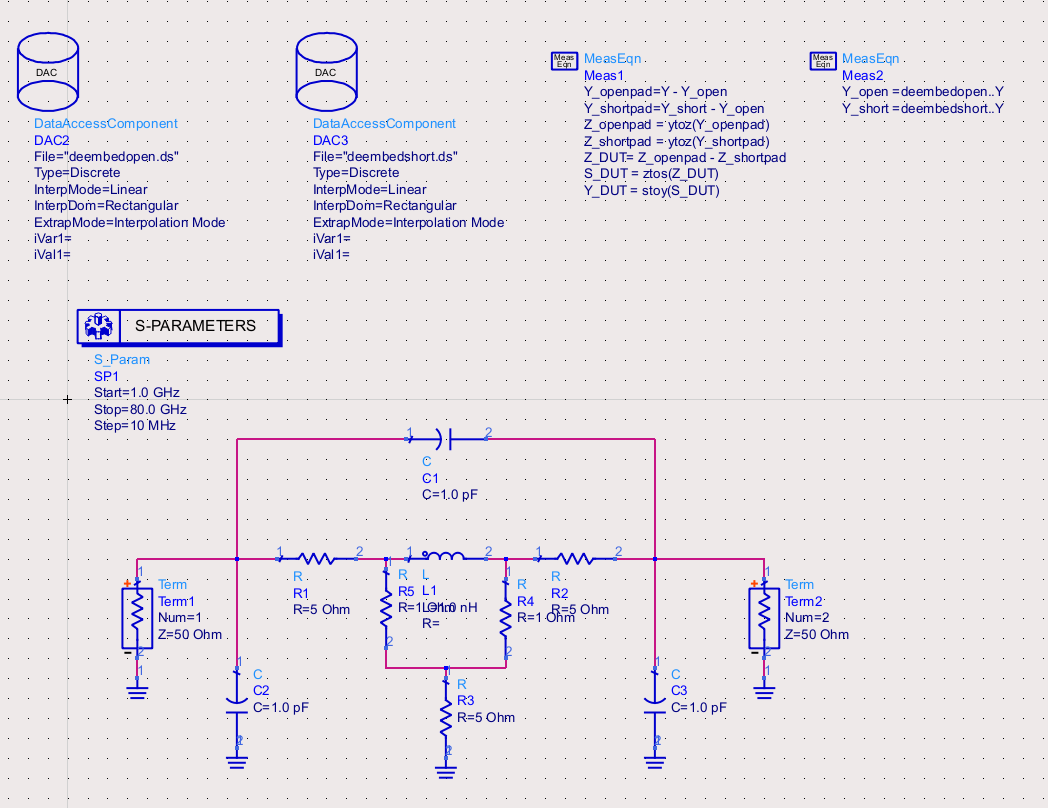
\includegraphics[scale=0.40]{de_embedding_whole.png}
  \caption{De-embedding : \'etape g\'en\'erale}
  \label{de-embedding-whole}
\end{center}
\end{figure}

Les r\'esultats de simulations du de-embedding (fig. \ref{de-embedding-whole-sim}) montre le comportement avec parasite (premier rang),
et celui en de-embedded (sans parasite, deuxi\`eme rang).

\begin{figure}[!htb]
\begin{center}
  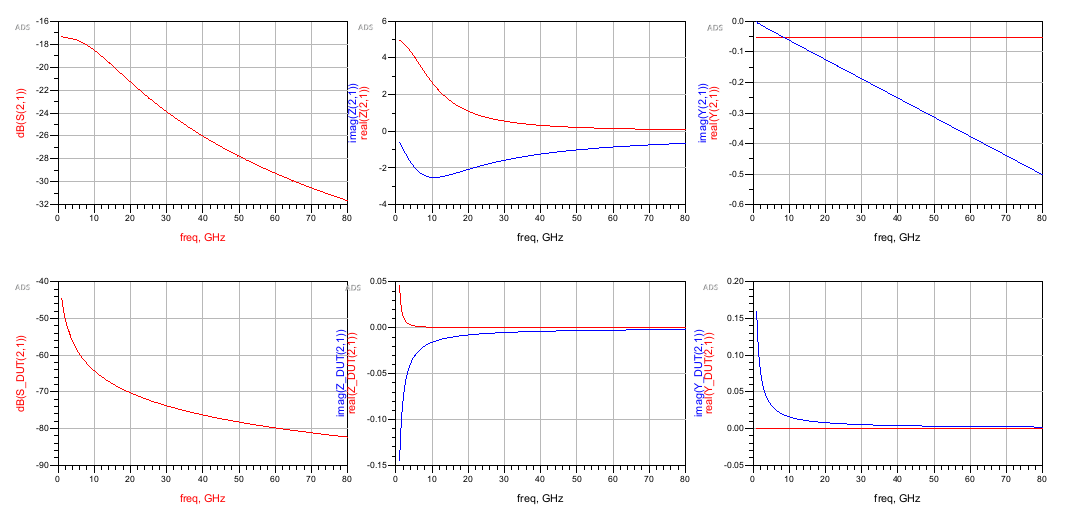
\includegraphics[scale=0.40]{de-embedding_whole_sim.png}
  \caption{R\'esultats de simulations de-embedding}
  \label{de-embedding-whole-sim}
\end{center}
\end{figure}

Ces deux r\'esultats sont compl\`etement diff\'erent : Les plots d'acc\`es ajoutes des distortions significatives qui peuvent compl\`etement
changer le fonctionnement du circuit (dans ce cas). Le sch\'ema \'equivalent en de-embedded - sans parasites - est certainement proche du celui
de la fig. \ref{de-embedding-bench}

\clearpage
\subsection{Comparaison avec un bench sans parasites}

On peut voir, en comparant les fig.\ref{de-embedding-whole-sim} et \ref{de-embedding-bench_sim}, que le comportement des deux sch\'emas (de-embedding
sans parasites et bench (sans plots d'acc\`es)), est identique.

\begin{figure}[!htb]
\begin{center}
  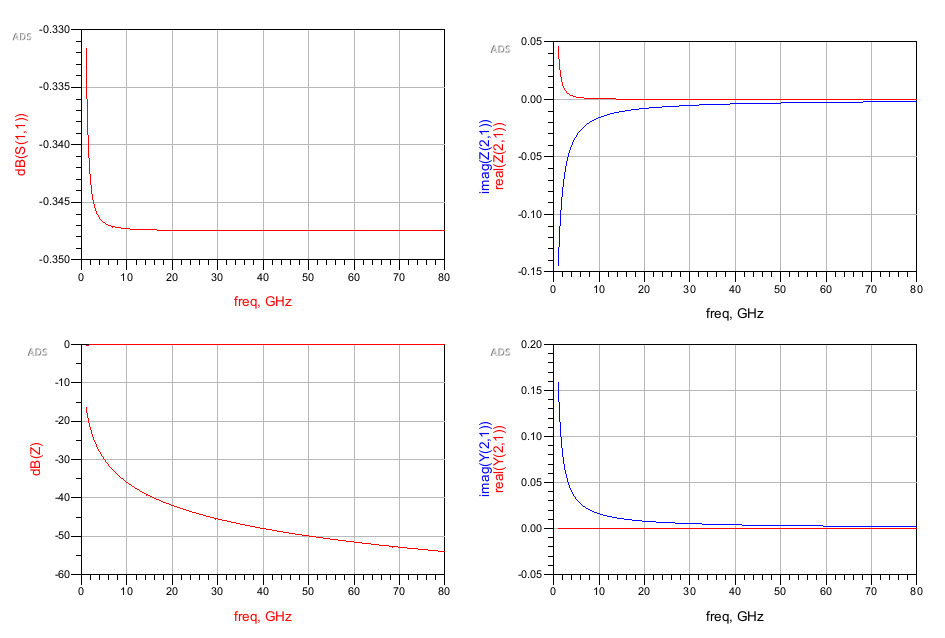
\includegraphics[scale=0.40]{de-embedding_bench_sim.png}
  \caption{Simulations du bench (sans parasites)}
  \label{de-embedding-bench_sim}
\end{center}
\end{figure}

\section{Conclusion}

Ces s\'eances de travaux pratiques sous ADS ont permis d'\'etudier la conception de filtres et
 d'antennes en technologie microruban telle qu'utilis\'ee actuellement dans l'industrie.

L'utilisation avanc\'ee de ce logiciel nous a amen\'e \`a effectuer des simulations de mod\`eles schematic et de mod\`ele layout, selon la m\'ethode des
 moments \'electromagn\'etiques, et \`a comparer ces simulations. Nous avons remarqu\'e \`a plusieurs reprises les influences des couplages capacitifs
parasites entre les lignes de propagation sur les performances d'adaptation du filtre, influences qui n'\'etaient pas pr\'esentes lors des simulations
du mod\`ele schematic.
Nous avons vu pour le filtre passe-bas et l'antenne que l'adaptation \`a $50 \Omega$ se faisait par des variations g\'eom\'etriques de longueur du layout.\\

Nous avons enfin vu comment coder sous forme logicielle les proc\'edures de deembedding avec la m\'ethode TRL qui permet de caract\'eriser un DUT sans les parasites li\'es aux pads.\\

Toutes ces techniques de design, mod\'elisation et de mesure des circuits RF sur l'outil logiciel ADS nous servira lors de la conception de
 l'\'emetteur-r\'ecepteur Wifi pour le projet 3A Syrf.

\clearpage
\addcontentsline{toc}{section}{R\'ef\'erences}

\begin{thebibliography}{9}

\bibitem{sim-elec-cours}
\textit{Simulation \'electromagn\'etique et techniques de mesure RF,}\\
\texttt{Jean-Daniel Arnould, Institut Polytechnique de Grenoble - Phelma}

\end{thebibliography}


\end{document}
